\documentclass[1p]{elsarticle_modified}
%\bibliographystyle{elsarticle-num}

%\usepackage[colorlinks]{hyperref}
%\usepackage{abbrmath_seonhwa} %\Abb, \Ascr, \Acal ,\Abf, \Afrak
\usepackage{amsfonts}
\usepackage{amssymb}
\usepackage{amsmath}
\usepackage{amsthm}
\usepackage{scalefnt}
\usepackage{amsbsy}
\usepackage{kotex}
\usepackage{caption}
\usepackage{subfig}
\usepackage{color}
\usepackage{graphicx}
\usepackage{xcolor} %% white, black, red, green, blue, cyan, magenta, yellow
\usepackage{float}
\usepackage{setspace}
\usepackage{hyperref}

\usepackage{tikz}
\usetikzlibrary{arrows}

\usepackage{multirow}
\usepackage{array} % fixed length table
\usepackage{hhline}

%%%%%%%%%%%%%%%%%%%%%
\makeatletter
\renewcommand*\env@matrix[1][\arraystretch]{%
	\edef\arraystretch{#1}%
	\hskip -\arraycolsep
	\let\@ifnextchar\new@ifnextchar
	\array{*\c@MaxMatrixCols c}}
\makeatother %https://tex.stackexchange.com/questions/14071/how-can-i-increase-the-line-spacing-in-a-matrix
%%%%%%%%%%%%%%%

\usepackage[normalem]{ulem}

\newcommand{\msout}[1]{\ifmmode\text{\sout{\ensuremath{#1}}}\else\sout{#1}\fi}
%SOURCE: \msout is \stkout macro in https://tex.stackexchange.com/questions/20609/strikeout-in-math-mode

\newcommand{\cancel}[1]{
	\ifmmode
	{\color{red}\msout{#1}}
	\else
	{\color{red}\sout{#1}}
	\fi
}

\newcommand{\add}[1]{
	{\color{blue}\uwave{#1}}
}

\newcommand{\replace}[2]{
	\ifmmode
	{\color{red}\msout{#1}}{\color{blue}\uwave{#2}}
	\else
	{\color{red}\sout{#1}}{\color{blue}\uwave{#2}}
	\fi
}

\newcommand{\Sol}{\mathcal{S}} %segment
\newcommand{\D}{D} %diagram
\newcommand{\A}{\mathcal{A}} %arc


%%%%%%%%%%%%%%%%%%%%%%%%%%%%%5 test

\def\sl{\operatorname{\textup{SL}}(2,\Cbb)}
\def\psl{\operatorname{\textup{PSL}}(2,\Cbb)}
\def\quan{\mkern 1mu \triangleright \mkern 1mu}

\theoremstyle{definition}
\newtheorem{thm}{Theorem}[section]
\newtheorem{prop}[thm]{Proposition}
\newtheorem{lem}[thm]{Lemma}
\newtheorem{ques}[thm]{Question}
\newtheorem{cor}[thm]{Corollary}
\newtheorem{defn}[thm]{Definition}
\newtheorem{exam}[thm]{Example}
\newtheorem{rmk}[thm]{Remark}
\newtheorem{alg}[thm]{Algorithm}

\newcommand{\I}{\sqrt{-1}}
\begin{document}

%\begin{frontmatter}
%
%\title{Boundary parabolic representations of knots up to 8 crossings}
%
%%% Group authors per affiliation:
%\author{Yunhi Cho} 
%\address{Department of Mathematics, University of Seoul, Seoul, Korea}
%\ead{yhcho@uos.ac.kr}
%
%
%\author{Seonhwa Kim} %\fnref{s_kim}}
%\address{Center for Geometry and Physics, Institute for Basic Science, Pohang, 37673, Korea}
%\ead{ryeona17@ibs.re.kr}
%
%\author{Hyuk Kim}
%\address{Department of Mathematical Sciences, Seoul National University, Seoul 08826, Korea}
%\ead{hyukkim@snu.ac.kr}
%
%\author{Seokbeom Yoon}
%\address{Department of Mathematical Sciences, Seoul National University, Seoul, 08826,  Korea}
%\ead{sbyoon15@snu.ac.kr}
%
%\begin{abstract}
%We find all boundary parabolic representation of knots up to 8 crossings.
%
%\end{abstract}
%\begin{keyword}
%    \MSC[2010] 57M25 
%\end{keyword}
%
%\end{frontmatter}

%\linenumbers
%\tableofcontents
%
\newcommand\colored[1]{\textcolor{white}{\rule[-0.35ex]{0.8em}{1.4ex}}\kern-0.8em\color{red} #1}%
%\newcommand\colored[1]{\textcolor{white}{ #1}\kern-2.17ex	\textcolor{white}{ #1}\kern-1.81ex	\textcolor{white}{ #1}\kern-2.15ex\color{red}#1	}

{\Large $\underline{12a_{0052}~(K12a_{0052})}$}

\setlength{\tabcolsep}{10pt}
\renewcommand{\arraystretch}{1.6}
\vspace{1cm}\begin{tabular}{m{100pt}>{\centering\arraybackslash}m{274pt}}
\multirow{5}{120pt}{
	\centering
	\includegraphics[width=112pt]{../../../GIT/diagram.site/Diagrams/png/853_12a_0052.png}\\
\ \ \ A knot diagram\footnotemark}&
\allowdisplaybreaks
\textbf{Linearized knot diagam} \\
\cline{2-2}
 &
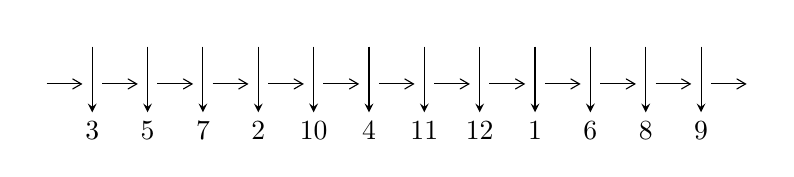
\begin{tikzpicture}[x=20pt, y=17pt]
	% nodes
	\node (C0) at (0, 0) {};
	\node (C1) at (1, 0) {};
	\node (C1U) at (1, +1) {};
	\node (C1D) at (1, -1) {3};

	\node (C2) at (2, 0) {};
	\node (C2U) at (2, +1) {};
	\node (C2D) at (2, -1) {5};

	\node (C3) at (3, 0) {};
	\node (C3U) at (3, +1) {};
	\node (C3D) at (3, -1) {7};

	\node (C4) at (4, 0) {};
	\node (C4U) at (4, +1) {};
	\node (C4D) at (4, -1) {2};

	\node (C5) at (5, 0) {};
	\node (C5U) at (5, +1) {};
	\node (C5D) at (5, -1) {10};

	\node (C6) at (6, 0) {};
	\node (C6U) at (6, +1) {};
	\node (C6D) at (6, -1) {4};

	\node (C7) at (7, 0) {};
	\node (C7U) at (7, +1) {};
	\node (C7D) at (7, -1) {11};

	\node (C8) at (8, 0) {};
	\node (C8U) at (8, +1) {};
	\node (C8D) at (8, -1) {12};

	\node (C9) at (9, 0) {};
	\node (C9U) at (9, +1) {};
	\node (C9D) at (9, -1) {1};

	\node (C10) at (10, 0) {};
	\node (C10U) at (10, +1) {};
	\node (C10D) at (10, -1) {6};

	\node (C11) at (11, 0) {};
	\node (C11U) at (11, +1) {};
	\node (C11D) at (11, -1) {8};

	\node (C12) at (12, 0) {};
	\node (C12U) at (12, +1) {};
	\node (C12D) at (12, -1) {9};
	\node (C13) at (13, 0) {};

	% arrows
	\draw[->,>={angle 60}]
	(C0) edge (C1) (C1) edge (C2) (C2) edge (C3) (C3) edge (C4) (C4) edge (C5) (C5) edge (C6) (C6) edge (C7) (C7) edge (C8) (C8) edge (C9) (C9) edge (C10) (C10) edge (C11) (C11) edge (C12) (C12) edge (C13) ;	\draw[->,>=stealth]
	(C1U) edge (C1D) (C2U) edge (C2D) (C3U) edge (C3D) (C4U) edge (C4D) (C5U) edge (C5D) (C6U) edge (C6D) (C7U) edge (C7D) (C8U) edge (C8D) (C9U) edge (C9D) (C10U) edge (C10D) (C11U) edge (C11D) (C12U) edge (C12D) ;
	\end{tikzpicture} \\
\hhline{~~} \\& 
\textbf{Solving Sequence} \\ \cline{2-2} 
 &
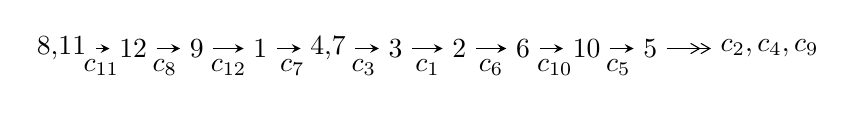
\begin{tikzpicture}[x=23pt, y=7pt]
	% node
	\node (A0) at (-1/8, 0) {8,11};
	\node (A1) at (1, 0) {12};
	\node (A2) at (2, 0) {9};
	\node (A3) at (3, 0) {1};
	\node (A4) at (65/16, 0) {4,7};
	\node (A5) at (41/8, 0) {3};
	\node (A6) at (49/8, 0) {2};
	\node (A7) at (57/8, 0) {6};
	\node (A8) at (65/8, 0) {10};
	\node (A9) at (73/8, 0) {5};
	\node (C1) at (1/2, -1) {$c_{11}$};
	\node (C2) at (3/2, -1) {$c_{8}$};
	\node (C3) at (5/2, -1) {$c_{12}$};
	\node (C4) at (7/2, -1) {$c_{7}$};
	\node (C5) at (37/8, -1) {$c_{3}$};
	\node (C6) at (45/8, -1) {$c_{1}$};
	\node (C7) at (53/8, -1) {$c_{6}$};
	\node (C8) at (61/8, -1) {$c_{10}$};
	\node (C9) at (69/8, -1) {$c_{5}$};
	\node (A10) at (11, 0) {$c_{2},c_{4},c_{9}$};

	% edge
	\draw[->,>=stealth]	
	(A0) edge (A1) (A1) edge (A2) (A2) edge (A3) (A3) edge (A4) (A4) edge (A5) (A5) edge (A6) (A6) edge (A7) (A7) edge (A8) (A8) edge (A9) ;
	\draw[->>,>={angle 60}]	
	(A9) edge (A10);
\end{tikzpicture} \\ 

\end{tabular} \\

\footnotetext{
The image of knot diagram is generated by the software ``\textbf{Draw programme}" developed by Andrew Bartholomew(\url{http://www.layer8.co.uk/maths/draw/index.htm\#Running-draw}), where we modified some parts for our purpose(\url{https://github.com/CATsTAILs/LinksPainter}).
}\phantom \\ \newline 
\centering \textbf{Ideals for irreducible components\footnotemark of $X_{\text{par}}$} 
 
\begin{align*}
I^u_{1}&=\langle 
1.62429\times10^{21} u^{62}+5.48543\times10^{21} u^{61}+\cdots+1.76821\times10^{20} b-1.09318\times10^{21},\\
\phantom{I^u_{1}}&\phantom{= \langle  }1.33327\times10^{20} u^{62}+3.96132\times10^{20} u^{61}+\cdots+1.76821\times10^{20} a+5.67190\times10^{20},\;u^{63}+5 u^{62}+\cdots-8 u-1\rangle \\
I^u_{2}&=\langle 
7 a^2 u-4 a^2-9 a u+61 b-21 a+46 u-35,\;a^3+a^2 u+a^2- a u+6 a+5 u+2,\;u^2- u-1\rangle \\
I^u_{3}&=\langle 
u^2+b+u-2,\;u^2+a+u-2,\;u^3+u^2-2 u-1\rangle \\
\\
\end{align*}
\raggedright * 3 irreducible components of $\dim_{\mathbb{C}}=0$, with total 72 representations.\\
\footnotetext{All coefficients of polynomials are rational numbers. But the coefficients are sometimes approximated in decimal forms when there is not enough margin.}
\newpage
\renewcommand{\arraystretch}{1}
\centering \section*{I. $I^u_{1}= \langle 1.62\times10^{21} u^{62}+5.49\times10^{21} u^{61}+\cdots+1.77\times10^{20} b-1.09\times10^{21},\;1.33\times10^{20} u^{62}+3.96\times10^{20} u^{61}+\cdots+1.77\times10^{20} a+5.67\times10^{20},\;u^{63}+5 u^{62}+\cdots-8 u-1 \rangle$}
\flushleft \textbf{(i) Arc colorings}\\
\begin{tabular}{m{7pt} m{180pt} m{7pt} m{180pt} }
\flushright $a_{8}=$&$\begin{pmatrix}0\\u\end{pmatrix}$ \\
\flushright $a_{11}=$&$\begin{pmatrix}1\\0\end{pmatrix}$ \\
\flushright $a_{12}=$&$\begin{pmatrix}1\\u^2\end{pmatrix}$ \\
\flushright $a_{9}=$&$\begin{pmatrix}- u\\- u^3+u\end{pmatrix}$ \\
\flushright $a_{1}=$&$\begin{pmatrix}- u^2+1\\- u^4+2 u^2\end{pmatrix}$ \\
\flushright $a_{4}=$&$\begin{pmatrix}-0.754022 u^{62}-2.24030 u^{61}+\cdots-21.4495 u-3.20771\\-9.18606 u^{62}-31.0226 u^{61}+\cdots+46.9211 u+6.18243\end{pmatrix}$ \\
\flushright $a_{7}=$&$\begin{pmatrix}u\\u\end{pmatrix}$ \\
\flushright $a_{3}=$&$\begin{pmatrix}-23.4953 u^{62}-77.2375 u^{61}+\cdots+77.1418 u+10.1702\\-31.9273 u^{62}-106.020 u^{61}+\cdots+145.512 u+19.5604\end{pmatrix}$ \\
\flushright $a_{2}=$&$\begin{pmatrix}-10.7523 u^{62}-35.7397 u^{61}+\cdots+57.9187 u+7.96787\\-2.43432 u^{62}-7.52201 u^{61}+\cdots+4.03934 u+0.358011\end{pmatrix}$ \\
\flushright $a_{6}=$&$\begin{pmatrix}24.0607 u^{62}+78.4765 u^{61}+\cdots-116.822 u-16.4195\\20.0955 u^{62}+65.6712 u^{61}+\cdots-84.1906 u-11.8348\end{pmatrix}$ \\
\flushright $a_{10}=$&$\begin{pmatrix}u^3-2 u\\u^5-3 u^3+u\end{pmatrix}$ \\
\flushright $a_{5}=$&$\begin{pmatrix}-13.0012 u^{62}-42.0114 u^{61}+\cdots+38.8447 u+4.43096\\-21.3192 u^{62}-70.2291 u^{61}+\cdots+92.7241 u+12.0408\end{pmatrix}$\\&\end{tabular}
\flushleft \textbf{(ii) Obstruction class $= -1$}\\~\\
\flushleft \textbf{(iii) Cusp Shapes $= -\frac{910404764759386405011}{29470106428947974938} u^{62}-\frac{3960180972357089673875}{29470106428947974938} u^{61}+\cdots+\frac{9246140476465749326853}{29470106428947974938} u+\frac{1190469186010506308511}{29470106428947974938}$}\\~\\
\newpage\renewcommand{\arraystretch}{1}
\flushleft \textbf{(iv) u-Polynomials at the component}\newline \\
\begin{tabular}{m{50pt}|m{274pt}}
Crossings & \hspace{64pt}u-Polynomials at each crossing \\
\hline $$\begin{aligned}c_{1}\end{aligned}$$&$\begin{aligned}
&u^{63}+32 u^{62}+\cdots+328 u+1
\end{aligned}$\\
\hline $$\begin{aligned}c_{2},c_{4}\end{aligned}$$&$\begin{aligned}
&u^{63}-6 u^{62}+\cdots+12 u+1
\end{aligned}$\\
\hline $$\begin{aligned}c_{3},c_{6}\end{aligned}$$&$\begin{aligned}
&u^{63}-3 u^{62}+\cdots-20 u+8
\end{aligned}$\\
\hline $$\begin{aligned}c_{5},c_{10}\end{aligned}$$&$\begin{aligned}
&u^{63}-2 u^{62}+\cdots-224 u-64
\end{aligned}$\\
\hline $$\begin{aligned}c_{7},c_{8},c_{9}\\c_{11},c_{12}\end{aligned}$$&$\begin{aligned}
&u^{63}+5 u^{62}+\cdots-8 u-1
\end{aligned}$\\
\hline
\end{tabular}\\~\\
\newpage\renewcommand{\arraystretch}{1}
\flushleft \textbf{(v) Riley Polynomials at the component}\newline \\
\begin{tabular}{m{50pt}|m{274pt}}
Crossings & \hspace{64pt}Riley Polynomials at each crossing \\
\hline $$\begin{aligned}c_{1}\end{aligned}$$&$\begin{aligned}
&y^{63}+4 y^{62}+\cdots+101996 y-1
\end{aligned}$\\
\hline $$\begin{aligned}c_{2},c_{4}\end{aligned}$$&$\begin{aligned}
&y^{63}-32 y^{62}+\cdots+328 y-1
\end{aligned}$\\
\hline $$\begin{aligned}c_{3},c_{6}\end{aligned}$$&$\begin{aligned}
&y^{63}+27 y^{62}+\cdots+1872 y-64
\end{aligned}$\\
\hline $$\begin{aligned}c_{5},c_{10}\end{aligned}$$&$\begin{aligned}
&y^{63}-40 y^{62}+\cdots+160768 y-4096
\end{aligned}$\\
\hline $$\begin{aligned}c_{7},c_{8},c_{9}\\c_{11},c_{12}\end{aligned}$$&$\begin{aligned}
&y^{63}-85 y^{62}+\cdots-52 y-1
\end{aligned}$\\
\hline
\end{tabular}\\~\\
\newpage\flushleft \textbf{(vi) Complex Volumes and Cusp Shapes}
$$\begin{array}{c|c|c}  
\text{Solutions to }I^u_{1}& \I (\text{vol} + \sqrt{-1}CS) & \text{Cusp shape}\\
 \hline 
\begin{aligned}
u &= \phantom{-}1.028890 + 0.152703 I \\
a &= \phantom{-}0.905018 - 0.380951 I \\
b &= \phantom{-}0.0268490 + 0.0773734 I\end{aligned}
 & -4.77176 - 0.89078 I & \phantom{-0.000000 } 0 \\ \hline\begin{aligned}
u &= \phantom{-}1.028890 - 0.152703 I \\
a &= \phantom{-}0.905018 + 0.380951 I \\
b &= \phantom{-}0.0268490 - 0.0773734 I\end{aligned}
 & -4.77176 + 0.89078 I & \phantom{-0.000000 } 0 \\ \hline\begin{aligned}
u &= \phantom{-}0.999217 + 0.355880 I \\
a &= -0.49337 + 1.91103 I \\
b &= -1.42854 + 1.09253 I\end{aligned}
 & -2.32837 - 6.62955 I & \phantom{-0.000000 } 0 \\ \hline\begin{aligned}
u &= \phantom{-}0.999217 - 0.355880 I \\
a &= -0.49337 - 1.91103 I \\
b &= -1.42854 - 1.09253 I\end{aligned}
 & -2.32837 + 6.62955 I & \phantom{-0.000000 } 0 \\ \hline\begin{aligned}
u &= -0.896327 + 0.253744 I \\
a &= -0.749447 - 0.960775 I \\
b &= -1.295060 - 0.092213 I\end{aligned}
 & \phantom{-}0.036006 + 1.082630 I & \phantom{-0.000000 } 0 \\ \hline\begin{aligned}
u &= -0.896327 - 0.253744 I \\
a &= -0.749447 + 0.960775 I \\
b &= -1.295060 + 0.092213 I\end{aligned}
 & \phantom{-}0.036006 - 1.082630 I & \phantom{-0.000000 } 0 \\ \hline\begin{aligned}
u &= -1.055640 + 0.212243 I \\
a &= \phantom{-}0.668837 + 0.903910 I \\
b &= \phantom{-}1.341030 + 0.052198 I\end{aligned}
 & -1.79480 + 5.60016 I & \phantom{-0.000000 } 0 \\ \hline\begin{aligned}
u &= -1.055640 - 0.212243 I \\
a &= \phantom{-}0.668837 - 0.903910 I \\
b &= \phantom{-}1.341030 - 0.052198 I\end{aligned}
 & -1.79480 - 5.60016 I & \phantom{-0.000000 } 0 \\ \hline\begin{aligned}
u &= \phantom{-}1.044900 + 0.298813 I \\
a &= -0.829234 + 0.625125 I \\
b &= -0.059797 - 0.170377 I\end{aligned}
 & -6.88408 - 5.57625 I & \phantom{-0.000000 } 0 \\ \hline\begin{aligned}
u &= \phantom{-}1.044900 - 0.298813 I \\
a &= -0.829234 - 0.625125 I \\
b &= -0.059797 + 0.170377 I\end{aligned}
 & -6.88408 + 5.57625 I & \phantom{-0.000000 } 0\\
 \hline 
 \end{array}$$\newpage$$\begin{array}{c|c|c}  
\text{Solutions to }I^u_{1}& \I (\text{vol} + \sqrt{-1}CS) & \text{Cusp shape}\\
 \hline 
\begin{aligned}
u &= \phantom{-}1.063910 + 0.242269 I \\
a &= \phantom{-}0.77322 - 2.30918 I \\
b &= \phantom{-}1.43939 - 1.55305 I\end{aligned}
 & -7.53862 - 2.77757 I & \phantom{-0.000000 } 0 \\ \hline\begin{aligned}
u &= \phantom{-}1.063910 - 0.242269 I \\
a &= \phantom{-}0.77322 + 2.30918 I \\
b &= \phantom{-}1.43939 + 1.55305 I\end{aligned}
 & -7.53862 + 2.77757 I & \phantom{-0.000000 } 0 \\ \hline\begin{aligned}
u &= -0.886505 + 0.065475 I \\
a &= \phantom{-}0.866237 - 0.584689 I \\
b &= \phantom{-}1.55540 + 0.00724 I\end{aligned}
 & -3.50514 + 0.98775 I & \phantom{-0.000000 } 0 \\ \hline\begin{aligned}
u &= -0.886505 - 0.065475 I \\
a &= \phantom{-}0.866237 + 0.584689 I \\
b &= \phantom{-}1.55540 - 0.00724 I\end{aligned}
 & -3.50514 - 0.98775 I & \phantom{-0.000000 } 0 \\ \hline\begin{aligned}
u &= \phantom{-}1.048840 + 0.413504 I \\
a &= \phantom{-}0.60788 - 1.71015 I \\
b &= \phantom{-}1.60656 - 1.01476 I\end{aligned}
 & -5.14579 - 12.09490 I & \phantom{-0.000000 } 0 \\ \hline\begin{aligned}
u &= \phantom{-}1.048840 - 0.413504 I \\
a &= \phantom{-}0.60788 + 1.71015 I \\
b &= \phantom{-}1.60656 + 1.01476 I\end{aligned}
 & -5.14579 + 12.09490 I & \phantom{-0.000000 } 0 \\ \hline\begin{aligned}
u &= -0.559821 + 0.591306 I \\
a &= \phantom{-}0.608474 + 1.194700 I \\
b &= \phantom{-}0.988829 - 0.154158 I\end{aligned}
 & -2.11826 - 4.21827 I & -12.00000 + 0. I\phantom{ +0.000000I} \\ \hline\begin{aligned}
u &= -0.559821 - 0.591306 I \\
a &= \phantom{-}0.608474 - 1.194700 I \\
b &= \phantom{-}0.988829 + 0.154158 I\end{aligned}
 & -2.11826 + 4.21827 I & -12.00000 + 0. I\phantom{ +0.000000I} \\ \hline\begin{aligned}
u &= \phantom{-}0.801660 + 0.061483 I \\
a &= \phantom{-}0.08712 + 2.74634 I \\
b &= -0.240999 + 0.989685 I\end{aligned}
 & \phantom{-}1.61353 - 3.07418 I & -21.7450 + 6.3725 I \\ \hline\begin{aligned}
u &= \phantom{-}0.801660 - 0.061483 I \\
a &= \phantom{-}0.08712 - 2.74634 I \\
b &= -0.240999 - 0.989685 I\end{aligned}
 & \phantom{-}1.61353 + 3.07418 I & -21.7450 - 6.3725 I\\
 \hline 
 \end{array}$$\newpage$$\begin{array}{c|c|c}  
\text{Solutions to }I^u_{1}& \I (\text{vol} + \sqrt{-1}CS) & \text{Cusp shape}\\
 \hline 
\begin{aligned}
u &= -0.626636 + 0.416140 I \\
a &= -0.724621 - 1.147740 I \\
b &= -1.018610 - 0.016299 I\end{aligned}
 & \phantom{-}0.0003302 + 0.0283867 I & -12.00000 - 1.58557 I \\ \hline\begin{aligned}
u &= -0.626636 - 0.416140 I \\
a &= -0.724621 + 1.147740 I \\
b &= -1.018610 + 0.016299 I\end{aligned}
 & \phantom{-}0.0003302 - 0.0283867 I & -12.00000 + 1.58557 I \\ \hline\begin{aligned}
u &= -0.240977 + 0.680886 I \\
a &= \phantom{-}0.303437 - 0.160247 I \\
b &= -1.41332 - 0.53392 I\end{aligned}
 & -1.15974 + 8.39259 I & -13.8921 - 7.9238 I \\ \hline\begin{aligned}
u &= -0.240977 - 0.680886 I \\
a &= \phantom{-}0.303437 + 0.160247 I \\
b &= -1.41332 + 0.53392 I\end{aligned}
 & -1.15974 - 8.39259 I & -13.8921 + 7.9238 I \\ \hline\begin{aligned}
u &= \phantom{-}1.309330 + 0.213784 I \\
a &= -0.511554 + 0.626098 I \\
b &= -0.244470 - 0.005554 I\end{aligned}
 & -8.22487 + 1.35085 I & \phantom{-0.000000 } 0 \\ \hline\begin{aligned}
u &= \phantom{-}1.309330 - 0.213784 I \\
a &= -0.511554 - 0.626098 I \\
b &= -0.244470 + 0.005554 I\end{aligned}
 & -8.22487 - 1.35085 I & \phantom{-0.000000 } 0 \\ \hline\begin{aligned}
u &= -0.181089 + 0.593484 I \\
a &= -0.476070 + 0.258477 I \\
b &= \phantom{-}1.33722 + 0.54379 I\end{aligned}
 & \phantom{-}1.31779 + 3.40957 I & -9.77047 - 4.49596 I \\ \hline\begin{aligned}
u &= -0.181089 - 0.593484 I \\
a &= -0.476070 - 0.258477 I \\
b &= \phantom{-}1.33722 - 0.54379 I\end{aligned}
 & \phantom{-}1.31779 - 3.40957 I & -9.77047 + 4.49596 I \\ \hline\begin{aligned}
u &= -0.275760 + 0.524784 I \\
a &= \phantom{-}0.59469 + 1.49476 I \\
b &= \phantom{-}0.752601 - 0.186307 I\end{aligned}
 & -2.78020 + 2.76904 I & -15.9302 - 5.0017 I \\ \hline\begin{aligned}
u &= -0.275760 - 0.524784 I \\
a &= \phantom{-}0.59469 - 1.49476 I \\
b &= \phantom{-}0.752601 + 0.186307 I\end{aligned}
 & -2.78020 - 2.76904 I & -15.9302 + 5.0017 I\\
 \hline 
 \end{array}$$\newpage$$\begin{array}{c|c|c}  
\text{Solutions to }I^u_{1}& \I (\text{vol} + \sqrt{-1}CS) & \text{Cusp shape}\\
 \hline 
\begin{aligned}
u &= -0.362579 + 0.450678 I \\
a &= \phantom{-}0.062756 - 0.676284 I \\
b &= -1.43437 - 0.73425 I\end{aligned}
 & -3.12199 + 0.43767 I & -16.9567 - 5.0899 I \\ \hline\begin{aligned}
u &= -0.362579 - 0.450678 I \\
a &= \phantom{-}0.062756 + 0.676284 I \\
b &= -1.43437 + 0.73425 I\end{aligned}
 & -3.12199 - 0.43767 I & -16.9567 + 5.0899 I \\ \hline\begin{aligned}
u &= -0.546898\phantom{ +0.000000I} \\
a &= -3.12245\phantom{ +0.000000I} \\
b &= -3.56875\phantom{ +0.000000I}\end{aligned}
 & -2.45024\phantom{ +0.000000I} & -97.9560\phantom{ +0.000000I} \\ \hline\begin{aligned}
u &= \phantom{-}0.127965 + 0.446646 I \\
a &= -1.274990 - 0.311863 I \\
b &= \phantom{-}1.060070 + 0.298515 I\end{aligned}
 & \phantom{-}3.14642 + 1.35383 I & -6.03722 - 2.02193 I \\ \hline\begin{aligned}
u &= \phantom{-}0.127965 - 0.446646 I \\
a &= -1.274990 + 0.311863 I \\
b &= \phantom{-}1.060070 - 0.298515 I\end{aligned}
 & \phantom{-}3.14642 - 1.35383 I & -6.03722 + 2.02193 I \\ \hline\begin{aligned}
u &= \phantom{-}0.300748 + 0.343620 I \\
a &= \phantom{-}1.44873 + 1.07671 I \\
b &= -0.909905 - 0.082810 I\end{aligned}
 & \phantom{-}2.43021 - 3.64228 I & -6.61693 + 6.48458 I \\ \hline\begin{aligned}
u &= \phantom{-}0.300748 - 0.343620 I \\
a &= \phantom{-}1.44873 - 1.07671 I \\
b &= -0.909905 + 0.082810 I\end{aligned}
 & \phantom{-}2.43021 + 3.64228 I & -6.61693 - 6.48458 I \\ \hline\begin{aligned}
u &= \phantom{-}1.55975 + 0.08766 I \\
a &= \phantom{-}0.524965 - 1.191820 I \\
b &= \phantom{-}0.600823 - 0.640135 I\end{aligned}
 & -7.43465 - 1.76582 I & \phantom{-0.000000 } 0 \\ \hline\begin{aligned}
u &= \phantom{-}1.55975 - 0.08766 I \\
a &= \phantom{-}0.524965 + 1.191820 I \\
b &= \phantom{-}0.600823 + 0.640135 I\end{aligned}
 & -7.43465 + 1.76582 I & \phantom{-0.000000 } 0 \\ \hline\begin{aligned}
u &= \phantom{-}1.61037\phantom{ +0.000000I} \\
a &= \phantom{-}3.62252\phantom{ +0.000000I} \\
b &= \phantom{-}3.92432\phantom{ +0.000000I}\end{aligned}
 & -10.1147\phantom{ +0.000000I} & \phantom{-0.000000 } 0\\
 \hline 
 \end{array}$$\newpage$$\begin{array}{c|c|c}  
\text{Solutions to }I^u_{1}& \I (\text{vol} + \sqrt{-1}CS) & \text{Cusp shape}\\
 \hline 
\begin{aligned}
u &= -0.381909\phantom{ +0.000000I} \\
a &= -1.00049\phantom{ +0.000000I} \\
b &= -0.382079\phantom{ +0.000000I}\end{aligned}
 & -0.657964\phantom{ +0.000000I} & -14.9870\phantom{ +0.000000I} \\ \hline\begin{aligned}
u &= -1.68795 + 0.01367 I \\
a &= \phantom{-}0.14081 + 2.60287 I \\
b &= \phantom{-}0.23802 + 1.66652 I\end{aligned}
 & -7.35150 + 3.34536 I & \phantom{-0.000000 } 0 \\ \hline\begin{aligned}
u &= -1.68795 - 0.01367 I \\
a &= \phantom{-}0.14081 - 2.60287 I \\
b &= \phantom{-}0.23802 - 1.66652 I\end{aligned}
 & -7.35150 - 3.34536 I & \phantom{-0.000000 } 0 \\ \hline\begin{aligned}
u &= \phantom{-}1.69104 + 0.05015 I \\
a &= \phantom{-}1.24766 - 1.01147 I \\
b &= \phantom{-}1.58417 - 0.51110 I\end{aligned}
 & -9.10013 - 2.17742 I & \phantom{-0.000000 } 0 \\ \hline\begin{aligned}
u &= \phantom{-}1.69104 - 0.05015 I \\
a &= \phantom{-}1.24766 + 1.01147 I \\
b &= \phantom{-}1.58417 + 0.51110 I\end{aligned}
 & -9.10013 + 2.17742 I & \phantom{-0.000000 } 0 \\ \hline\begin{aligned}
u &= \phantom{-}1.70113 + 0.01268 I \\
a &= -1.57689 - 0.79292 I \\
b &= -2.02027 - 0.39058 I\end{aligned}
 & -12.78410 - 1.26409 I & \phantom{-0.000000 } 0 \\ \hline\begin{aligned}
u &= \phantom{-}1.70113 - 0.01268 I \\
a &= -1.57689 + 0.79292 I \\
b &= -2.02027 + 0.39058 I\end{aligned}
 & -12.78410 + 1.26409 I & \phantom{-0.000000 } 0 \\ \hline\begin{aligned}
u &= -1.72001 + 0.09428 I \\
a &= \phantom{-}1.03143 + 2.22415 I \\
b &= \phantom{-}1.49512 + 1.52284 I\end{aligned}
 & -11.9480 + 8.4481 I & \phantom{-0.000000 } 0 \\ \hline\begin{aligned}
u &= -1.72001 - 0.09428 I \\
a &= \phantom{-}1.03143 - 2.22415 I \\
b &= \phantom{-}1.49512 - 1.52284 I\end{aligned}
 & -11.9480 - 8.4481 I & \phantom{-0.000000 } 0 \\ \hline\begin{aligned}
u &= -1.72905 + 0.04304 I \\
a &= -0.288124 - 0.148815 I \\
b &= \phantom{-}0.389884 + 0.095224 I\end{aligned}
 & -14.6550 + 1.7190 I & \phantom{-0.000000 } 0\\
 \hline 
 \end{array}$$\newpage$$\begin{array}{c|c|c}  
\text{Solutions to }I^u_{1}& \I (\text{vol} + \sqrt{-1}CS) & \text{Cusp shape}\\
 \hline 
\begin{aligned}
u &= -1.72905 - 0.04304 I \\
a &= -0.288124 + 0.148815 I \\
b &= \phantom{-}0.389884 - 0.095224 I\end{aligned}
 & -14.6550 - 1.7190 I & \phantom{-0.000000 } 0 \\ \hline\begin{aligned}
u &= -1.73268 + 0.07792 I \\
a &= \phantom{-}0.239402 + 0.232586 I \\
b &= -0.419372 - 0.168398 I\end{aligned}
 & -16.7785 + 7.1236 I & \phantom{-0.000000 } 0 \\ \hline\begin{aligned}
u &= -1.73268 - 0.07792 I \\
a &= \phantom{-}0.239402 - 0.232586 I \\
b &= -0.419372 + 0.168398 I\end{aligned}
 & -16.7785 - 7.1236 I & \phantom{-0.000000 } 0 \\ \hline\begin{aligned}
u &= -1.73373 + 0.11357 I \\
a &= -1.20066 - 2.06097 I \\
b &= -1.72265 - 1.40659 I\end{aligned}
 & -14.9724 + 14.2765 I & \phantom{-0.000000 } 0 \\ \hline\begin{aligned}
u &= -1.73373 - 0.11357 I \\
a &= -1.20066 + 2.06097 I \\
b &= -1.72265 + 1.40659 I\end{aligned}
 & -14.9724 - 14.2765 I & \phantom{-0.000000 } 0 \\ \hline\begin{aligned}
u &= -1.73663 + 0.06289 I \\
a &= -1.09099 - 2.68531 I \\
b &= -1.42955 - 2.04344 I\end{aligned}
 & -17.5514 + 4.0414 I & \phantom{-0.000000 } 0 \\ \hline\begin{aligned}
u &= -1.73663 - 0.06289 I \\
a &= -1.09099 + 2.68531 I \\
b &= -1.42955 + 2.04344 I\end{aligned}
 & -17.5514 - 4.0414 I & \phantom{-0.000000 } 0 \\ \hline\begin{aligned}
u &= \phantom{-}1.73782 + 0.05723 I \\
a &= -1.19559 + 0.80808 I \\
b &= -1.60415 + 0.24819 I\end{aligned}
 & -11.81270 - 6.72860 I & \phantom{-0.000000 } 0 \\ \hline\begin{aligned}
u &= \phantom{-}1.73782 - 0.05723 I \\
a &= -1.19559 - 0.80808 I \\
b &= -1.60415 - 0.24819 I\end{aligned}
 & -11.81270 + 6.72860 I & \phantom{-0.000000 } 0 \\ \hline\begin{aligned}
u &= -1.80049 + 0.02971 I \\
a &= \phantom{-}0.095999 + 0.111650 I \\
b &= -0.178594 - 0.166882 I\end{aligned}
 & -19.6506 - 0.4097 I & \phantom{-0.000000 } 0\\
 \hline 
 \end{array}$$\newpage$$\begin{array}{c|c|c}  
\text{Solutions to }I^u_{1}& \I (\text{vol} + \sqrt{-1}CS) & \text{Cusp shape}\\
 \hline 
\begin{aligned}
u &= -1.80049 - 0.02971 I \\
a &= \phantom{-}0.095999 - 0.111650 I \\
b &= -0.178594 + 0.166882 I\end{aligned}
 & -19.6506 + 0.4097 I & \phantom{-0.000000 } 0 \\ \hline\begin{aligned}
u &= -0.030116 + 0.163245 I \\
a &= -1.54490 - 3.56904 I \\
b &= -0.483050 + 0.114818 I\end{aligned}
 & -0.977525 - 0.103718 I & -10.13328 - 1.14919 I \\ \hline\begin{aligned}
u &= -0.030116 - 0.163245 I \\
a &= -1.54490 + 3.56904 I \\
b &= -0.483050 - 0.114818 I\end{aligned}
 & -0.977525 + 0.103718 I & -10.13328 + 1.14919 I\\
 \hline 
 \end{array}$$\newpage\newpage\renewcommand{\arraystretch}{1}
\centering \section*{II. $I^u_{2}= \langle 7 a^2 u-4 a^2-9 a u+61 b-21 a+46 u-35,\;a^3+a^2 u+a^2- a u+6 a+5 u+2,\;u^2- u-1 \rangle$}
\flushleft \textbf{(i) Arc colorings}\\
\begin{tabular}{m{7pt} m{180pt} m{7pt} m{180pt} }
\flushright $a_{8}=$&$\begin{pmatrix}0\\u\end{pmatrix}$ \\
\flushright $a_{11}=$&$\begin{pmatrix}1\\0\end{pmatrix}$ \\
\flushright $a_{12}=$&$\begin{pmatrix}1\\u+1\end{pmatrix}$ \\
\flushright $a_{9}=$&$\begin{pmatrix}- u\\- u-1\end{pmatrix}$ \\
\flushright $a_{1}=$&$\begin{pmatrix}- u\\- u\end{pmatrix}$ \\
\flushright $a_{4}=$&$\begin{pmatrix}a\\-0.114754 a^{2} u+0.147541 a u+\cdots+0.344262 a+0.573770\end{pmatrix}$ \\
\flushright $a_{7}=$&$\begin{pmatrix}u\\u\end{pmatrix}$ \\
\flushright $a_{3}=$&$\begin{pmatrix}-0.163934 a^{2} u-0.360656 a u+\cdots+0.491803 a-0.180328\\-0.278689 a^{2} u-0.213115 a u+\cdots-0.163934 a+0.393443\end{pmatrix}$ \\
\flushright $a_{2}=$&$\begin{pmatrix}0.0163934 a^{2} u-0.163934 a u+\cdots-0.0491803 a-0.0819672\\-0.278689 a^{2} u-0.213115 a u+\cdots-0.163934 a+0.393443\end{pmatrix}$ \\
\flushright $a_{6}=$&$\begin{pmatrix}0.295082 a^{2} u+0.0491803 a u+\cdots+0.114754 a-0.475410\\0\end{pmatrix}$ \\
\flushright $a_{10}=$&$\begin{pmatrix}1\\0\end{pmatrix}$ \\
\flushright $a_{5}=$&$\begin{pmatrix}0.295082 a^{2} u+0.0491803 a u+\cdots+0.114754 a-0.475410\\0\end{pmatrix}$\\&\end{tabular}
\flushleft \textbf{(ii) Obstruction class $= 1$}\\~\\
\flushleft \textbf{(iii) Cusp Shapes $= \frac{93}{61} a^2 u-\frac{27}{61} a^2+\frac{46}{61} a u+\frac{26}{61} a+\frac{341}{61} u-\frac{831}{61}$}\\~\\
\newpage\renewcommand{\arraystretch}{1}
\flushleft \textbf{(iv) u-Polynomials at the component}\newline \\
\begin{tabular}{m{50pt}|m{274pt}}
Crossings & \hspace{64pt}u-Polynomials at each crossing \\
\hline $$\begin{aligned}c_{1},c_{3}\end{aligned}$$&$\begin{aligned}
&(u^3- u^2+2 u-1)^2
\end{aligned}$\\
\hline $$\begin{aligned}c_{2}\end{aligned}$$&$\begin{aligned}
&(u^3+u^2-1)^2
\end{aligned}$\\
\hline $$\begin{aligned}c_{4}\end{aligned}$$&$\begin{aligned}
&(u^3- u^2+1)^2
\end{aligned}$\\
\hline $$\begin{aligned}c_{5},c_{10}\end{aligned}$$&$\begin{aligned}
&u^6
\end{aligned}$\\
\hline $$\begin{aligned}c_{6}\end{aligned}$$&$\begin{aligned}
&(u^3+u^2+2 u+1)^2
\end{aligned}$\\
\hline $$\begin{aligned}c_{7},c_{8},c_{9}\end{aligned}$$&$\begin{aligned}
&(u^2+u-1)^3
\end{aligned}$\\
\hline $$\begin{aligned}c_{11},c_{12}\end{aligned}$$&$\begin{aligned}
&(u^2- u-1)^3
\end{aligned}$\\
\hline
\end{tabular}\\~\\
\newpage\renewcommand{\arraystretch}{1}
\flushleft \textbf{(v) Riley Polynomials at the component}\newline \\
\begin{tabular}{m{50pt}|m{274pt}}
Crossings & \hspace{64pt}Riley Polynomials at each crossing \\
\hline $$\begin{aligned}c_{1},c_{3},c_{6}\end{aligned}$$&$\begin{aligned}
&(y^3+3 y^2+2 y-1)^2
\end{aligned}$\\
\hline $$\begin{aligned}c_{2},c_{4}\end{aligned}$$&$\begin{aligned}
&(y^3- y^2+2 y-1)^2
\end{aligned}$\\
\hline $$\begin{aligned}c_{5},c_{10}\end{aligned}$$&$\begin{aligned}
&y^6
\end{aligned}$\\
\hline $$\begin{aligned}c_{7},c_{8},c_{9}\\c_{11},c_{12}\end{aligned}$$&$\begin{aligned}
&(y^2-3 y+1)^3
\end{aligned}$\\
\hline
\end{tabular}\\~\\
\newpage\flushleft \textbf{(vi) Complex Volumes and Cusp Shapes}
$$\begin{array}{c|c|c}  
\text{Solutions to }I^u_{2}& \I (\text{vol} + \sqrt{-1}CS) & \text{Cusp shape}\\
 \hline 
\begin{aligned}
u &= -0.618034\phantom{ +0.000000I} \\
a &= \phantom{-}0.162553\phantom{ +0.000000I} \\
b &= \phantom{-}1.08457\phantom{ +0.000000I}\end{aligned}
 & -2.10041\phantom{ +0.000000I} & -17.1210\phantom{ +0.000000I} \\ \hline\begin{aligned}
u &= -0.618034\phantom{ +0.000000I} \\
a &= -0.27226 + 2.57535 I \\
b &= \phantom{-}0.075747 + 0.460350 I\end{aligned}
 & \phantom{-}2.03717 + 2.82812 I & -7.98462 + 1.83947 I \\ \hline\begin{aligned}
u &= -0.618034\phantom{ +0.000000I} \\
a &= -0.27226 - 2.57535 I \\
b &= \phantom{-}0.075747 - 0.460350 I\end{aligned}
 & \phantom{-}2.03717 - 2.82812 I & -7.98462 - 1.83947 I \\ \hline\begin{aligned}
u &= \phantom{-}1.61803\phantom{ +0.000000I} \\
a &= -0.06538 + 2.01307 I \\
b &= -0.198308 + 1.205210 I\end{aligned}
 & -5.85852 - 2.82812 I & -12.87990 + 2.78145 I \\ \hline\begin{aligned}
u &= \phantom{-}1.61803\phantom{ +0.000000I} \\
a &= -0.06538 - 2.01307 I \\
b &= -0.198308 - 1.205210 I\end{aligned}
 & -5.85852 + 2.82812 I & -12.87990 - 2.78145 I \\ \hline\begin{aligned}
u &= \phantom{-}1.61803\phantom{ +0.000000I} \\
a &= -2.48727\phantom{ +0.000000I} \\
b &= -2.83945\phantom{ +0.000000I}\end{aligned}
 & -9.99610\phantom{ +0.000000I} & \phantom{-}3.85000\phantom{ +0.000000I}\\
 \hline 
 \end{array}$$\newpage\newpage\renewcommand{\arraystretch}{1}
\centering \section*{III. $I^u_{3}= \langle u^2+b+u-2,\;u^2+a+u-2,\;u^3+u^2-2 u-1 \rangle$}
\flushleft \textbf{(i) Arc colorings}\\
\begin{tabular}{m{7pt} m{180pt} m{7pt} m{180pt} }
\flushright $a_{8}=$&$\begin{pmatrix}0\\u\end{pmatrix}$ \\
\flushright $a_{11}=$&$\begin{pmatrix}1\\0\end{pmatrix}$ \\
\flushright $a_{12}=$&$\begin{pmatrix}1\\u^2\end{pmatrix}$ \\
\flushright $a_{9}=$&$\begin{pmatrix}- u\\u^2- u-1\end{pmatrix}$ \\
\flushright $a_{1}=$&$\begin{pmatrix}- u^2+1\\- u^2+u+1\end{pmatrix}$ \\
\flushright $a_{4}=$&$\begin{pmatrix}- u^2- u+2\\- u^2- u+2\end{pmatrix}$ \\
\flushright $a_{7}=$&$\begin{pmatrix}u\\u\end{pmatrix}$ \\
\flushright $a_{3}=$&$\begin{pmatrix}- u^2- u+2\\- u^2- u+2\end{pmatrix}$ \\
\flushright $a_{2}=$&$\begin{pmatrix}-2 u^2- u+3\\-2 u^2+3\end{pmatrix}$ \\
\flushright $a_{6}=$&$\begin{pmatrix}u\\u\end{pmatrix}$ \\
\flushright $a_{10}=$&$\begin{pmatrix}- u^2+1\\- u^2\end{pmatrix}$ \\
\flushright $a_{5}=$&$\begin{pmatrix}u^2-1\\u^2- u-1\end{pmatrix}$\\&\end{tabular}
\flushleft \textbf{(ii) Obstruction class $= 1$}\\~\\
\flushleft \textbf{(iii) Cusp Shapes $= -8 u^2-7 u+2$}\\~\\
\newpage\renewcommand{\arraystretch}{1}
\flushleft \textbf{(iv) u-Polynomials at the component}\newline \\
\begin{tabular}{m{50pt}|m{274pt}}
Crossings & \hspace{64pt}u-Polynomials at each crossing \\
\hline $$\begin{aligned}c_{1},c_{2}\end{aligned}$$&$\begin{aligned}
&(u-1)^3
\end{aligned}$\\
\hline $$\begin{aligned}c_{3},c_{6}\end{aligned}$$&$\begin{aligned}
&u^3
\end{aligned}$\\
\hline $$\begin{aligned}c_{4}\end{aligned}$$&$\begin{aligned}
&(u+1)^3
\end{aligned}$\\
\hline $$\begin{aligned}c_{5},c_{7},c_{8}\\c_{9}\end{aligned}$$&$\begin{aligned}
&u^3- u^2-2 u+1
\end{aligned}$\\
\hline $$\begin{aligned}c_{10},c_{11},c_{12}\end{aligned}$$&$\begin{aligned}
&u^3+u^2-2 u-1
\end{aligned}$\\
\hline
\end{tabular}\\~\\
\newpage\renewcommand{\arraystretch}{1}
\flushleft \textbf{(v) Riley Polynomials at the component}\newline \\
\begin{tabular}{m{50pt}|m{274pt}}
Crossings & \hspace{64pt}Riley Polynomials at each crossing \\
\hline $$\begin{aligned}c_{1},c_{2},c_{4}\end{aligned}$$&$\begin{aligned}
&(y-1)^3
\end{aligned}$\\
\hline $$\begin{aligned}c_{3},c_{6}\end{aligned}$$&$\begin{aligned}
&y^3
\end{aligned}$\\
\hline $$\begin{aligned}c_{5},c_{7},c_{8}\\c_{9},c_{10},c_{11}\\c_{12}\end{aligned}$$&$\begin{aligned}
&y^3-5 y^2+6 y-1
\end{aligned}$\\
\hline
\end{tabular}\\~\\
\newpage\flushleft \textbf{(vi) Complex Volumes and Cusp Shapes}
$$\begin{array}{c|c|c}  
\text{Solutions to }I^u_{3}& \I (\text{vol} + \sqrt{-1}CS) & \text{Cusp shape}\\
 \hline 
\begin{aligned}
u &= \phantom{-}1.24698\phantom{ +0.000000I} \\
a &= -0.801938\phantom{ +0.000000I} \\
b &= -0.801938\phantom{ +0.000000I}\end{aligned}
 & -7.98968\phantom{ +0.000000I} & -19.1690\phantom{ +0.000000I} \\ \hline\begin{aligned}
u &= -0.445042\phantom{ +0.000000I} \\
a &= \phantom{-}2.24698\phantom{ +0.000000I} \\
b &= \phantom{-}2.24698\phantom{ +0.000000I}\end{aligned}
 & -2.34991\phantom{ +0.000000I} & \phantom{-}3.53080\phantom{ +0.000000I} \\ \hline\begin{aligned}
u &= -1.80194\phantom{ +0.000000I} \\
a &= \phantom{-}0.554958\phantom{ +0.000000I} \\
b &= \phantom{-}0.554958\phantom{ +0.000000I}\end{aligned}
 & -19.2692\phantom{ +0.000000I} & -11.3620\phantom{ +0.000000I}\\
 \hline 
 \end{array}$$\newpage
\newpage\renewcommand{\arraystretch}{1}
\centering \section*{ IV. u-Polynomials}
\begin{tabular}{m{50pt}|m{274pt}}
Crossings & \hspace{64pt}u-Polynomials at each crossing \\
\hline $$\begin{aligned}c_{1}\end{aligned}$$&$\begin{aligned}
&((u-1)^3)(u^3- u^2+2 u-1)^2(u^{63}+32 u^{62}+\cdots+328 u+1)
\end{aligned}$\\
\hline $$\begin{aligned}c_{2}\end{aligned}$$&$\begin{aligned}
&((u-1)^3)(u^3+u^2-1)^2(u^{63}-6 u^{62}+\cdots+12 u+1)
\end{aligned}$\\
\hline $$\begin{aligned}c_{3}\end{aligned}$$&$\begin{aligned}
&u^3(u^3- u^2+2 u-1)^2(u^{63}-3 u^{62}+\cdots-20 u+8)
\end{aligned}$\\
\hline $$\begin{aligned}c_{4}\end{aligned}$$&$\begin{aligned}
&((u+1)^3)(u^3- u^2+1)^2(u^{63}-6 u^{62}+\cdots+12 u+1)
\end{aligned}$\\
\hline $$\begin{aligned}c_{5}\end{aligned}$$&$\begin{aligned}
&u^6(u^3- u^2-2 u+1)(u^{63}-2 u^{62}+\cdots-224 u-64)
\end{aligned}$\\
\hline $$\begin{aligned}c_{6}\end{aligned}$$&$\begin{aligned}
&u^3(u^3+u^2+2 u+1)^2(u^{63}-3 u^{62}+\cdots-20 u+8)
\end{aligned}$\\
\hline $$\begin{aligned}c_{7},c_{8},c_{9}\end{aligned}$$&$\begin{aligned}
&((u^2+u-1)^3)(u^3- u^2-2 u+1)(u^{63}+5 u^{62}+\cdots-8 u-1)
\end{aligned}$\\
\hline $$\begin{aligned}c_{10}\end{aligned}$$&$\begin{aligned}
&u^6(u^3+u^2-2 u-1)(u^{63}-2 u^{62}+\cdots-224 u-64)
\end{aligned}$\\
\hline $$\begin{aligned}c_{11},c_{12}\end{aligned}$$&$\begin{aligned}
&((u^2- u-1)^3)(u^3+u^2-2 u-1)(u^{63}+5 u^{62}+\cdots-8 u-1)
\end{aligned}$\\
\hline
\end{tabular}\newpage\renewcommand{\arraystretch}{1}
\centering \section*{ V. Riley Polynomials}
\begin{tabular}{m{50pt}|m{274pt}}
Crossings & \hspace{64pt}Riley Polynomials at each crossing \\
\hline $$\begin{aligned}c_{1}\end{aligned}$$&$\begin{aligned}
&((y-1)^3)(y^3+3 y^2+2 y-1)^2(y^{63}+4 y^{62}+\cdots+101996 y-1)
\end{aligned}$\\
\hline $$\begin{aligned}c_{2},c_{4}\end{aligned}$$&$\begin{aligned}
&((y-1)^3)(y^3- y^2+2 y-1)^2(y^{63}-32 y^{62}+\cdots+328 y-1)
\end{aligned}$\\
\hline $$\begin{aligned}c_{3},c_{6}\end{aligned}$$&$\begin{aligned}
&y^3(y^3+3 y^2+2 y-1)^2(y^{63}+27 y^{62}+\cdots+1872 y-64)
\end{aligned}$\\
\hline $$\begin{aligned}c_{5},c_{10}\end{aligned}$$&$\begin{aligned}
&y^6(y^3-5 y^2+6 y-1)(y^{63}-40 y^{62}+\cdots+160768 y-4096)
\end{aligned}$\\
\hline $$\begin{aligned}c_{7},c_{8},c_{9}\\c_{11},c_{12}\end{aligned}$$&$\begin{aligned}
&((y^2-3 y+1)^3)(y^3-5 y^2+6 y-1)(y^{63}-85 y^{62}+\cdots-52 y-1)
\end{aligned}$\\
\hline
\end{tabular}
\vskip 2pc
\end{document}